\chapter{Problemanalyse} \label{cha:problemanalyse}

\section{Anforderungen und Problemabgrenzung} \label{cha:problemanalyse:abgrenzung}

Die Schnitzeljagden sollen in erster Linie den Studienanfängern dienen, um ihnen auf interaktive Weise den Campus nahe zu bringen und sie mit den wichtigsten Orten und Einrichtungen vertraut zu machen.

Im Rahmen des Projekts wurden folgende Ziele in einer Vier-Felder-Matrix aufgeteilt.

\begin{figure}[H]
    \centering
    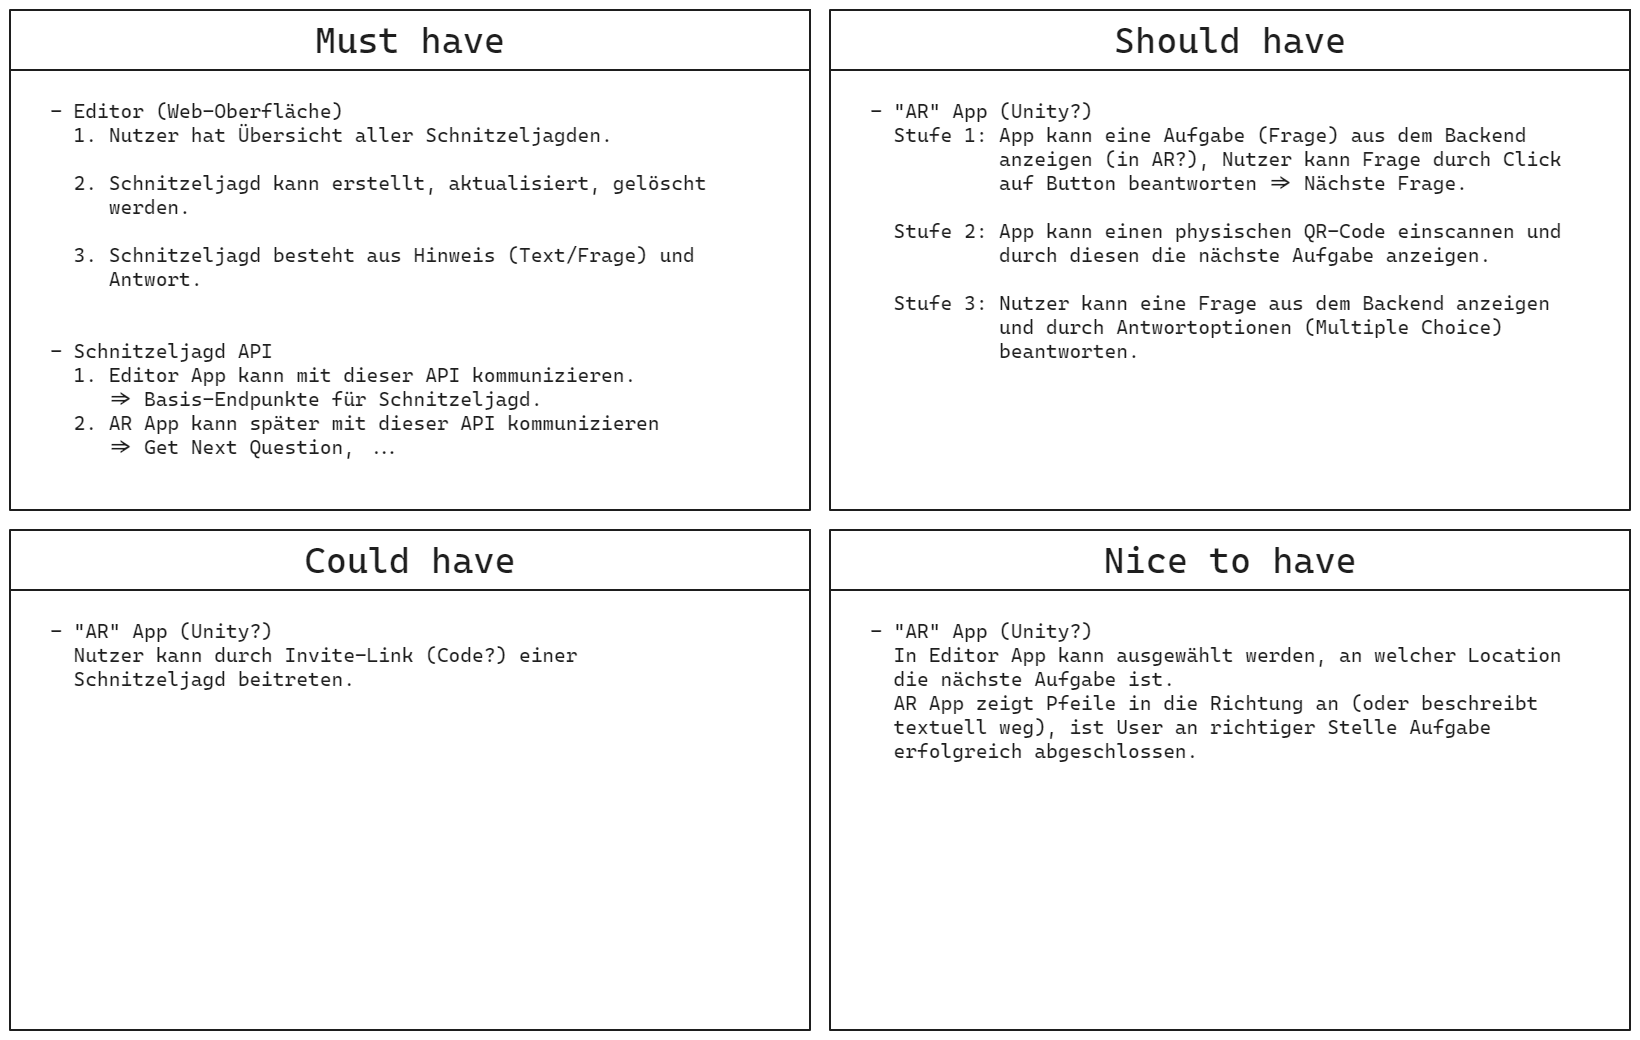
\includegraphics[width=\textwidth]{images/PrAr_ProblemAnalysis_Vierfelder.png}
    \caption{Darstellung der Projekt-Ziele aufgeteilt in Vier Felder}
    \label{fig:problemanalyse:vierfeldermatrixamarsch}
\end{figure}

Für die erfolgreiche Projektumsetzung sind folgende Eigenschaften zu berücksichtigen.

\subsubsection{Flexibilität}

Ein wichtiger Aspekt des Projektes ist, dass eine Schnitzeljagd so flexibel wie möglich umgesetzt werden soll. Aufgabenstellung und Lösung sollen voneinander entkoppelt und ohne großen Implementierungsaufwand dynamisch erweiterbar sein.

\subsubsection{Skalierbarkeit}

Das System muss in der Lage sein, mehrere Schnitzeljagden gleichzeitig ohne Probleme durchzuführen. Es sollte möglich sein, die Ressourcen des Systems dynamisch an die Anzahl der gerade aktiven Benutzer anzupassen, ohne dass es zu Leistungseinbußen oder ähnlichen Beeinträchtigungen kommt.

\subsubsection{Benutzerfreundlichkeit}

Der Anmelde- und der Durchführungsprozess sollten unabhängig voneinander klar strukturiert sein, um den Benutzern eine reibungslose und intuitive Erfahrung zu bieten. Während der Schnitzeljagd sollten keine Schwierigkeiten auftreten. Die Schnitzeljagd sollte den Benutzern ein einzigartiges Erlebnis bieten, ohne sie durch unnötige oder ablenkende Elemente zu stören. Idealerweise fungiert die Anwendung als Schnittstelle zur Durchführung der Schnitzeljagd, wobei die Lösung der Aufgaben direkte Interaktionen im realen Leben erfordert.

Die digitale Plattform ermöglicht eine einfache Anmeldung und Durchführung der Schnitzeljagd, wodurch der organisatorische Aufwand minimiert und die Zugänglichkeit maximiert wird.

\subsubsection{Sicherheit}

Das Thema Sicherheit ist im Zusammenhang mit sensiblen Benutzerdaten wie Passwörtern sehr wichtig. Durch die im Kapitel \ref{cha:swentwurf} beschriebenen Architekturüberlegungen wäre es möglich, Benutzerdaten durch kryptographisch sichere Hashfunktionen zu speichern. Um den Projektumfang auf das Wesentliche zu reduzieren, wurde dies im Projekt nicht berücksichtigt.

\section{Architektonische Überlegungen}

Bei der Wahl einer angemessenen Architektur für das System sind viele Aspekte zu berücksichtigen, unter anderem die in Kapitel \ref{cha:problemanalyse:abgrenzung} genannten Eigenschaften.

In Kapitel \ref{cha:swentwurf} wird daher der service-orientierte Ansatz für den Entwurf der Software allumfassend beschrieben.
